\documentclass[10pt, letterpaper]{report}
% !TeX program = xelatex
%==================PREAMBOLO=======================%
\usepackage[utf8]{inputenc}
\usepackage{psvectorian}
\usepackage{pgfplots}
\usepackage[Rejne]{fncychap}
\usepackage[export]{adjustbox}
\usepackage[T1]{fontenc}
\usepackage{lmodern}
\usepackage[shortlabels]{enumitem}
\usepackage{moresize}
\usepackage{graphicx} % Required for inserting images
\usepackage{hyperref}
\usepackage{listings}
\usepackage[table,xcdraw]{xcolor}
\usepackage{amssymb}
\usepackage{amsmath}
\usepackage[italian]{babel}
\usepackage{nicefrac, xfrac}
\usepackage{tikz}
\usepackage{mathrsfs} 
\usepackage{titletoc}
\usepackage{fancyhdr}
\usepackage{psvectorian,lipsum}
\usepackage{fourier-orns}
\usepackage{lipsum}
\usepackage[paper=a4paper,left=25mm,right=25mm,bottom=25mm,top=25mm]{geometry}
\definecolor{light-gray}{gray}{0.95}
\definecolor{cop}{HTML}{f7ecd7}
\definecolor{copAut}{HTML}{ababab}
\definecolor{copAut2}{HTML}{c3c3e6}
\definecolor{purcop}{HTML}{d0d3db}
\definecolor{sapienza}{HTML}{660f1d}
\definecolor{lightSapienza}{HTML}{e3d3d5}
\definecolor{darkgreen}{HTML}{008000}
\definecolor{cartaRiciclata}{HTML}{fcfcf7}
\newcommand{\redText}[1]{\color{red}#1\color{black}}
\newcommand{\code}[1]{\colorbox{light-gray}{\texttt{#1}}}
\newcommand{\codee}[1]{\colorbox{white}{\texttt{#1}}}
\newcommand{\K}{{\mathbb K}}
\newcommand{\notimplies}{%
  \mathrel{{\ooalign{\hidewidth$\not\phantom{=}$\hidewidth\cr$\implies$}}}}
\newcommand{\flowerLine}{ \begin{center}\decofourleft\hphantom{ }\decoone\hphantom{ }\decofourright\hphantom{}\hphantom{aa}
\decofourleft\hphantom{ }\decoone\hphantom{ }\decofourright\hphantom{}\hphantom{aa}
\decofourleft\hphantom{ }\decoone\hphantom{ }\decofourright\hphantom{}\hphantom{aa}
\decofourleft\hphantom{ }\decoone\hphantom{ }\decofourright\hphantom{}\hphantom{aa} 
\decofourleft\hphantom{ }\decoone\hphantom{ }\decofourright\hphantom{}\hphantom{aa}
\decofourleft\hphantom{ }\decoone\hphantom{ }\decofourright\hphantom{}\hphantom{aa}
\decofourleft\hphantom{ }\decoone\hphantom{ }\decofourright\hphantom{}\hphantom{aa}
\decofourleft\hphantom{ }\decoone\hphantom{ }\decofourright\hphantom{}\hphantom{aa}
\decofourleft\hphantom{ }\decoone\hphantom{ }\decofourright\hphantom{}\hphantom{aa}
\end{center}}
\definecolor{g}{RGB}{60, 50, 50}
\newcommand{\textg}[1]{\color{g}{\textbf{#1}}\color{black}}
\newcommand{\teo}[1]{{\large\color{sapienza}\textbf{Teorema #1 :\hphantom{a}}}}
\newcommand{\defi}[1]{{\large\color{sapienza}\textbf{Definizione #1 :\hphantom{a}}}}
\newcommand{\claim}[1]{{\color{sapienza}\textbf{Claim #1 :\hphantom{a}}}}
\newcommand{\lemma}[1]{{\color{sapienza}\textbf{Lemma #1 :\hphantom{a}}}}
\newcommand{\dimo}[1]{{\color{sapienza}\textbf{Dimostrazione #1 :\hphantom{a}}}}
\newcommand{\prop}[1]{{\color{sapienza}\textbf{Proposizione #1 :\hphantom{a}}}}
\newcommand\greybox[1]{%
  \vskip\baselineskip%
  \par\noindent\colorbox{light-gray}{%
    \begin{minipage}{\textwidth}#1\end{minipage}%
  }%
  \vskip\baselineskip%
}
\newcommand\sapbox[1]{%
  \vskip\baselineskip%
  \par\noindent\colorbox{lightSapienza}{%
    \begin{minipage}{\textwidth}#1\end{minipage}%
  }%
  \vskip\baselineskip%
}

\newcommand{\Z}{{\mathbb Z}}
\newcommand{\blank}{{\sqcup}}
\newcommand{\R}{{\mathbb R}}
\newcommand{\N}{{\mathbb N}}
\newcommand{\C}{{\mathbb C}}
\newcommand{\Sn}{{\mathcal S_n}}
\newcommand{\An}{{\mathcal A_n}}
\newcommand{\E}{{\mathcal E}}
\newcommand{\B}{{\mathcal B}}
\newcommand{\mcm}{{\text{mcm}}}
\newcommand{\rg}{{\text{rg}}}
\newcommand{\ve}{{\bar v}}
\newcommand{\spaz}{{\text{\hphantom{aa}}}}
\newcommand{\MCD}{{\text{MCD}}}
\newcommand{\tc}{{\text{ tale che }}}
\newcommand{\supp}{{\text{Supp}}}
\newcommand{\acc}{\\\hphantom{}\\}
\newcommand{\aut}{{\text{Aut}}}
\newcommand{\Span}{{\text{Span}}}
\newcommand{\End}{{\text{End}}}
\newcommand{\cen}{{\text{Centro}}}
\newcommand{\norm}{{\unlhd}}
\newcommand{\ciclS}{{\left \langle }}
\newcommand{\ciclE}{{\right \rangle }}
\newcommand{\boxedMath}[1]{\begin{tabular}{|c|}\hline \texttt{#1} \\ \hline\end{tabular} :}
\newcommand{\shell}[1]{\colorbox{black}{\textcolor{white}{\texttt{#1}}}}
\newcommand{\eqImportante}[1]{\begin{center}\huge\lefthand\hphantom{a}
    \normalsize\texttt{#1}
    \hphantom{aaa}\huge\righthand\end{center}}

\fancyhf{}
\pagestyle{fancy}
\usepackage{pgf-pie}  
\usetikzlibrary{positioning}

\renewcommand{\headrule}{%
\vspace{-8pt}\hrulefill
\raisebox{-2.1pt}{\quad\decothreeleft\decotwo\decothreeright\quad}\hrulefill}

%sta roba serve per il codice C
\definecolor{mGreen}{rgb}{0,0.6,0}
\definecolor{mGray}{rgb}{0.5,0.5,0.5}
\definecolor{mPurple}{rgb}{0.58,0,0.82}
\definecolor{backgroundColour}{rgb}{0.95,0.95,0.92}

\lstdefinestyle{CStyle}{
    backgroundcolor=\color{backgroundColour},   
    commentstyle=\color{mGreen},
    keywordstyle=\color{magenta},
    numberstyle=\tiny\color{mGray},
    stringstyle=\color{mPurple},
    basicstyle=\footnotesize,
    breakatwhitespace=false,         
    breaklines=true,                 
    captionpos=b,                    
    keepspaces=true,                 
    numbers=left,                    
    numbersep=5pt,                  
    showspaces=false,                
    showstringspaces=false,
    showtabs=false,                  
    tabsize=2,
    language=C
}
\lstdefinestyle{CppStyle}{
    backgroundcolor=\color{backgroundColour},   
    commentstyle=\color{mGreen}\ttfamily,
    morecomment=[l][\color{magenta}]{\#}
    keywordstyle=\color{blue}\ttfamily,
    numberstyle=\tiny\color{mGray},
    stringstyle=\color{red}\ttfamily,
    basicstyle=\ttfamily,
    breakatwhitespace=false,         
    breaklines=true,                 
    captionpos=b,                    
    keepspaces=true,                 
    numbers=left,                    
    numbersep=5pt,                  
    showspaces=false,                
    showstringspaces=false,
    showtabs=false,                  
    tabsize=2,
    language=C
}
\lstset{language=C++,
                basicstyle=\ttfamily,
                keywordstyle=\color{blue}\ttfamily,
                stringstyle=\color{red}\ttfamily,
                commentstyle=\color{green}\ttfamily,
                morecomment=[l][\color{magenta}]{\#}
}
%fine roba che serve per il codice C
\usepackage{minted}
 %TOGLI COMMENTO SE USI XELATEX
%\usepackage{fontspec}
\title{Programmazione di Sistemi Multicore} %========TITOLO========%
\author{Marco Casu}
\date{\vspace{-5ex}}
\begin{document}

%==================COPERTINA=======================%
\begin{titlepage}
    \pagecolor{purcop}
\begin{center}
    %TOGLI COMMENTO SE USI XELATEX
   %\setmainfont{Palace Script MT}
   \Huge Marco Casu\acc
    %\setmainfont{Grand Casino}
     %TOGLI COMMENTO SE USI XELATEX
    %\setmainfont{h Halfroad}
    \HUGE \decothreeleft\hphantom{ }{\Huge\selectfont Programmazione di Sistemi Multicore}\hphantom{ }\decothreeright
     %TOGLI COMMENTO SE USI XELATEX
   % \setmainfont{Times New Roman}
\end{center}
\thispagestyle{empty}
\begin{figure}[h]
    \centering{
        %l'immagine deve avere una risoluzione 2048x2048
        
\includegraphics[width=1\textwidth ]{images/copertina.jpeg}
    }
\end{figure}
\vfill 
\centering 
\includegraphics[width=0.4\textwidth ]{../../preamble/Stemma_sapienza.png} \acc
\centering \Large \color{sapienza}Facoltà di Ingegneria dell'Informazione,
Informatica e Statistica\\
Dipartimento di Informatica
\end{titlepage}

%===================FINE COPERTINA======================%
\newpage
\pagecolor{cartaRiciclata}%\setmainfont{Algerian}
\large
Questo documento è distribuito sotto la licenza 
\color{blue}\href{https://www.gnu.org/licenses/fdl-1.3.txt}{GNU}\color{black},  
è un resoconto degli appunti (eventualmente integrati con libri di testo) tratti dalle lezioni del corso di Programmazione di Sistemi Multicore
\hphantom{a}per la laurea 
triennale in Informatica. Se dovessi notare errori, ti prego di segnalarmeli.
\newpage %\setmainfont{Times New Roman}
\normalsize
\tableofcontents 
\newpage

%==================FOOTER e HEADER=======================%
\fancyhf{}
\fancyhead[L]{\nouppercase{\leftmark}}
\fancyhead[R]{Sezione \thesection}
\fancyfoot[C]{\thepage}
\fancyfoot[L]{Appunti di Prog. di Sistemi Multicore}
\fancyfoot[R]{ Marco Casu}
%\fancyfoot[R]{\setmainfont{Palace Script MT}\huge Marco Casu \setmainfont{Times New Roman}}
%==================FOOTER e HEADER=======================%

%Ricorda del comando \flowerLine per separare le sottosezioni. Le sezioni si separano nelle diverse pagine

%==================INIZIO======================%

\chapter{Parallelismo : Motivazioni}
\section{Introduzione}
In una \textit{GPU} (Graphics Processing Unit), nota anche come scheda video, ci sono circa 
80 miliardi di transistor, e vengono utilizzate per allenare i grossi modelli di intelligenza 
artificiale, i quali necessitano migliaia di GPU, non è un caso se \textit{Nvidia} ad oggi, con 
il boom dell'IA, è una delle aziende più quotate al mondo. Le GPU, e la loro 
programmazione, sono uno fra i principali argomenti di questo corso.\acc 
L'evoluzione dell'hardware, ha portato i grossi sistemi di computazione, ad essere formati da 
svariate unità di calcolo piuttosto che una singola unità molto potente, i processori stessi di uso comune, 
ad oggi sono composti da più \textit{core}.\acc 
La legge di Moore riguarda una stima empirica che mette in correlazione lo scorrere del tempo con 
l'aumentare della potenza di calcolo dei processori, se inizialmente, a partire dagli anni 70, tale potenza 
raddoppiava ogni due anni, ad oggi tale andamento è andato rallentando, raggiungendo un 
incremento 1.5 in 10 anni.
\begin{center}
    \includegraphics[width=300pt]{images/processor_trend.eps}
\end{center}
L'obbiettivo di costruire calcolatori sempre più potenti è dipeso dalla necessità dell'Uomo 
di risolvere problemi sempre più complessi, come ad esempio, la risoluzione del genoma umano.\acc 
Il motivo per il quale non è possibile costruire processori monolitici sempre più potenti, risiede 
in un \textit{limite fisico} riguardante la densità massima possibile dei transistor in 
un chip.\begin{enumerate}
    \item transistor più piccoli $\longrightarrow$ processori più veloci
    \item processori più veloci $\longrightarrow$ aumento del consumo energetico 
    \item aumento del consumo energetico $\longrightarrow$ aumento del calore 
    \item aumento del calore $\longrightarrow$ problemi di inaffidabilità dei transistor
\end{enumerate}
\flowerLine
\section{Modelli di Parallelismo}
L'informatico che intende scrivere del codice per un sistema multicore, deve esplicitamente 
sfruttare i diversi core, limitandosi a scrivere un codice sequenziale, non starebbe sfruttando a pieno 
l'hardware a disposizione, rendendo il processo meno efficiente di quanto potrebbe essere.\acc 
La maggior parte delle volte, un algoritmo sequenziale, non può essere direttamente tradotto in un 
algoritmo parallelo, per questo bisogna scrivere il codice facendo riferimento all'hardware di 
destinazione. Si consideri adesso il seguente codice sequenziale, che ha lo scopo di sommare 
$n$ numeri dati in input.
\begin{lstlisting}[style=CStyle]
    sum = 0;
    for(i=0; i<n; i++){
        x = compute_next_value(...);
        sum += x;
    }
\end{lstlisting}
Si vuole rendere tale algoritmo parallelo, sapendo di essere a disposizione di $p$ core.
\begin{lstlisting}[style=CStyle]
    local_sum = 0;
    first_index = ...;
    last_index = ...;
    for(local_i=first_index; first_index<last_index; local_i++){
        local_x = compute_next_value(...);
        local_sum += local_x;
    }
\end{lstlisting}
In tale esempio, ogni core possiede le sue variabili private non condivise con gli altri core, 
ed esegue indipendentemente il blocco di codice. Ogni core conterrà la somma
parziale di $\nicefrac{n}{p}$ valori.\acc 
\textbf{Esempio} (24 numeri, 8 core) :\begin{center}
    valori : $1,4,3,\;\;\;9,2,8,\;\;\;5,1,1,\;\;\;6,2,7,\;\;\;2,5,0,\;\;\;4,1,8,\;\;\;6,5,1,\;\;\;2,3,9$\acc 
    \begin{tabular}{|l|l|l|l|l|l|l|l|l|}
        \hline
        \rowcolor[HTML]{C0C0C0} 
        core & 0 & 1 & 2 & 3 & 4 & 5 & 6 & 7 \\ \hline
        \texttt{local\_sum}    & 8 & 19 & 7 & 15 & 7 & 13 & 12 & 14 \\ \hline
        \end{tabular}
\end{center}
A questo punto, per ottenere la somma totale, vi sarà un core \textit{master} che riceverà le somme 
parziali da tutti gli altri core, per poi eseguire la somma finale.
\begin{lstlisting}[style=CStyle]
    if(master){
        sum = local_sum;
        for c : core{
            if(c!=self){
                sum += c.local_sum;
            }
        }
    }else{
        send local_sum to master;
    }
\end{lstlisting}
Dividere i dati per poi far eseguire la stessa computazione ai diversi nodi è la forma più semplice 
di parallelismo. La soluzione adottata non è ideale, in quanto, in seguito al calcolo delle somme 
parziali, tutti i core escluso il master non staranno eseguendo calcoli. Una possibile 
idea alternativa è di far si che a coppie i nodi si condividano le somme parziali per poi calcolarne 
una somma comune, sviluppando uno scambio di dati ad albero, come mostrato in figura \ref{fig:tree_cores}.
\begin{figure}[h!]
    \centering
    \includegraphics[width=280pt]{images/tree.eps}
    \caption{calcolo somme a coppie}
    \label{fig:tree_cores}
\end{figure}\acc
Possiamo identificare due tipi di parallelismo :\begin{itemize}
    \item \textbf{parallelismo dei task} : fra i core vengono divise diverse attività che vengono 
    svolte autonomamente.
    \item \textbf{parallelismo dei dati} : i dati da elaborare vengono divisi, ogni core eseguirà 
    la stessa computazione ma su una porzione diversa dei dati.
\end{itemize}
Quando si scrive un programma parallelo bisogna prestare attenzione alla \textit{sincronizzazione} dei 
processi, in quanto potrebbero dover accedere ad una stessa area di memoria. Risulta cruciale 
saper mettere in \textit{comunicazione} i vari core, e suddividere equamente il 
\textit{carico di lavoro} fra di essi. Verranno considerate 4 diverse tecnologie per la programmazione 
multicore : \begin{itemize}
    \item \textit{MPI} (Message Passing Interface) [ libreria ]
    \item \textit{Posix} Threads [ libreria ]
    \item \textit{OpenMP} [ libreria e compilatore ]
    \item \textit{CUDA} [ libreria e compilatore ]
\end{itemize}
La programmazione delle GPU richiederà un diverso compilatore, e non il solito \texttt{gcc}, in quanto 
l'architettura della scheda video differisce da quella del processore, e con essa le istruzioni.\acc
I sistemi paralleli possono essere categorizzati sotto vari aspetti.\begin{itemize}
    \item \textbf{shared memory} : Tutti i core accedono ad un'area di memoria comune. L'accesso 
    e la sincronizzazione vanno gestiti con cautela.
    \item \textbf{distributed memory} : Ogni core ha un area di memoria privata, e la comunicazione 
    avviene attraverso un apposito canale per lo scambio dei messaggi. 
\end{itemize}
\begin{figure}[h!]
    \centering
    \includegraphics[width=280pt]{images/sdmem.eps}
    \caption{modelli di parallelismo}
    \label{fig:sdmem}
\end{figure}
Vi è un altra suddivisione nei sistemi paralleli :\begin{itemize}
    \item \textbf{MIMD} : Ogni core ha una control unit indipendente, diversi core possono eseguire 
    diverse istruzioni nello stesso momento.
    \item \textbf{SIMD} : Vi è un singolo program counter per tutti i core, che eseguono in maniera 
    parallela le stesse istruzioni. Due core non possono eseguire operazioni diverse nello stesso momento.
\end{itemize}
Le GPU hanno una struttura \textit{SIMD}.\begin{center}
    \begin{tabular}{c|
        >{\columncolor[HTML]{EFEFEF}}c |
        >{\columncolor[HTML]{EFEFEF}}c |}
        \cline{2-3}
                                                           & \cellcolor[HTML]{C0C0C0}shared memory & \cellcolor[HTML]{C0C0C0}distributed memory \\ \hline
        \multicolumn{1}{|c|}{\cellcolor[HTML]{C0C0C0}SIMD} & CUDA                                  &                                            \\ \hline
        \multicolumn{1}{|c|}{\cellcolor[HTML]{C0C0C0}MIMD} & Pthreads/OpenMP/CUDA                  & MPI                                        \\ \hline
        \end{tabular}
\end{center}
Fin'ora sono stati utilizzati 3 termini chiave riguardante i tipi di programmazione,
 sebbene non vi sia una definizione comunemente accettata, 
la seguente verrà adottata in tale contesto : \begin{itemize}
    \item \textit{concorrente} : più processi sono attivi in uno stesso momento 
    \item \textit{parallela} : diverse entità cooperative che operano in maniera ravvicinata per 
    un obbiettivo comune.
    \item \textit{distribuita} : diverse entità cooperative.
\end{itemize}
La programmazione parallela o distribuita implica che sia anche concorrente, non è vero il contrario.
\end{document}
